\documentclass[a4paper,12pt]{article} % добавить leqno в [] для нумерации слева
\usepackage[a4paper,top=1.3cm,bottom=2cm,left=1.5cm,right=1.5cm,marginparwidth=0.75cm]{geometry}
%%% Работа с русским языком
\usepackage{cmap}					% поиск в PDF
\usepackage{mathtext} 				% русские буквы в фомулах
\usepackage[T2A]{fontenc}			% кодировка
\usepackage[utf8]{inputenc}			% кодировка исходного текста
\usepackage[english,russian]{babel}	% локализация и переносы

\usepackage{multirow}
\usepackage{graphicx}
\usepackage{mathtools}
\usepackage{wrapfig}
\usepackage{tabularx}
\usepackage{amssymb}
\usepackage{hyperref}
\usepackage[rgb]{xcolor}
\hypersetup{colorlinks=true,urlcolor=blue}
%% Шрифты
\usepackage{euscript}	 % Шрифт Евклид
\usepackage{amsmath}
\usepackage{mathtools}
%%% Заголовок
\author{Lokhmatov Arseniy}
\title{Лабораторная работа по общей физике}

\date{\today}
\begin{document}
\begin{titlepage}
    \newpage
    \begin{center}
    {\large МОСКОВСКИЙ ФИЗИКО-ТЕХНИЧЕСКИЙ ИНСТИТУТ (НАЦИОНАЛЬНЫЙ ИССЛЕДОВАТЕЛЬСКИЙ УНИВЕРСИТЕТ)}
    \vspace{1cm}

    {\largeФизтех-школа аэрокосмических технологий}
    \vspace{6em}
    \end{center}
    
    \vspace{1.2em}

    \begin{center}
    %\textsc{\textbf{}}
    \Large Лабораторная работа №4.2.3 \\
    Интерферометр Релея
    \linebreak
    \end{center}
    
    \vspace{11em}
    
    \begin{flushright}
                       {\large Работу выполнили\\
                       Лохматов Арсений Игоревич\\
                       Козярский Алексей Сергеевич\\
                       Б03-303 }
    \end{flushright}

    \vspace{\fill}

    \begin{center}
        
\includegraphics[width=0.2\linewidth]{dasr.png}
    \end{center}

    \begin{center}
    Долгопрудный, 2025
    \end{center}

    \end{titlepage}

\section{Теоретическая часть}

\paragraph{Цель работы:}ознакомление с интерференцией на двух щелях, устройством и принципом действия интерферометра Релея и с его применением для измерения показателей преломления газов.
\paragraph{В работе используются:}технический интерферометр ИТР-1, светофильтр, баллон с углекислым газом, сильфон, манометр, краны.

\paragraph{Экспериментальная установка.}Интерферометр Релея — прибор для измерения разности показателей преломления — основан на явлении дифракции света на двух параллельных щелях. Схема прибора представлена на рис. 1 в вертикальной и горизонтальной проекциях. Лампа накаливания $\text{Л}$ с помощью конденсора $K$ ярко освещает узкую входную щель $S$, расположенную в фокусе объектива $O_1$ (фокусное расстояние $f$). Коллиматор, состоящий из щели $S$) и объектива $O_1$, посылает параллельный пучок на диафрагму $D$ с двумя вертикальными щелями (расстояние между щелями $d$). Свет после двойной щели проходит кювету $L$, состоящую из двух одинаковых стеклянных камер, в которые вводятся исследуемые газы (в нашей установке — $CO_2$ или воздух). Кювета занимает только верхнюю часть пространства между объективами $O_1$ и $O_2$, длина кюветы $l$. За кюветой расположены две стеклянные пластинки $J$ (компенсатор Жамена, см. ниже) и пластинка $\text{П}$.

\begin{figure}[h]
    \begin{center}
        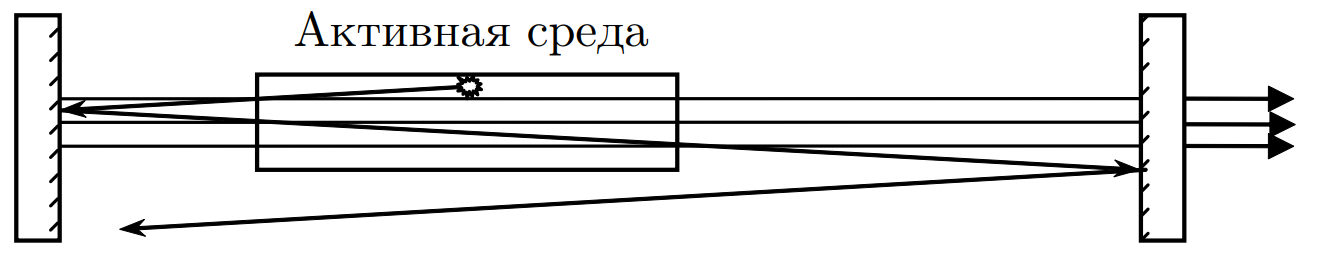
\includegraphics[width=15cm]{image1.png}
    \end{center}
    \caption{Устройство интерферометра Релея: a) вид сверху; б) вид сбоку}
    \label{img1}
\end{figure}

Интерференционная картина (картина дифракции на двух щелях), наблюдаемая в фокальной плоскости $F$ объектива $O_2$, представляет собой две системы равноотстоящих полос, параллельных щелям: верхняя (подвижная) образована лучами, прошедшими через кювету, нижняя (неподвижная) — лучами, прошедшими под кюветой. Обе системы интерференционных полос разграничены при помощи пластины II тонкой разделительной линией. Для наблюдения двух систем полос в окуляре применена цилиндрическая линза диаметром $2.2\text{ мм}$, ось которой расположена вертикально. Вторая («глазная») линза окуляра — обычная сферическая. Она служит для подстройки чёткости картины под глаз наблюдателя.

При малых дифракционных углах $\varphi = \lambda / d$ расстояние между соседними светлыми (или тёмными) полосами $\delta y$ зависит от длины волны $\lambda$, фокусного расстояния $f$ объектива $O_2$ и расстояния между дифракционными щелями $d$:

\[ \delta y = f \frac{\lambda}{d}. \]

В техническом интерферометре ИТР-1, который используется в нашей работе, $f \approx 20, \text{см}, d \approx 1.5, \text{см}, \delta y$  оказывается порядка $10^{-3} \, \text{см}$. Для наблюдения таких мелких интерференционных полос требуется окуляр с большим увеличением ($\gamma \approx 150^\circ$). Короткофокусная цилиндрическая линза окуляра $O$ сильно растягивает интерференционную картину по горизонтали, не меняя её вертикальных размеров и тем самым мало ослабляя освещённость полос. Изображение светящейся точки в фокальной плоскости объектива $O_2$ при рассматривании через цилиндрическую линзу имеет вид светлой вертикальной линии, длина которой определяется диаметром объектива. Поэтому распределение освещённости в нижней части светлой линии зависит от действия нижней части объектива, а в верхней части линии — от верхней части объектива. Таким образом, наблюдатель видит две системы полос: верхняя образована лучами, прошедшими через кюветы, нижняя — лучами, прошедшими под кюветами.

При заполнении камер газами с одинаковым показателем преломления $n$ обе системы полос совпадают. Оптическая разность хода $\Delta = \delta n \cdot l$, возникающая при прохождении света через камеры с разными газами $\delta n = n_2 - n_1$, ведёт к поперечному смещению верхней дифракционной картины относительно неподвижной нижней. Смещение на одну полосу соответствует дополнительной разности хода $\Delta = \lambda$. Просчитав число полос $m$ между центрами обеих картин, можно рассчитать

\[ \delta n = \frac{\Delta}{\ell} = m \frac{\lambda}{\ell}. \]

Для точного измерения разности хода используется компенсатор Жамена ($J$ на рисунке $\ref{img1}$) -- устройство, которое позволяет вернуть подвижную систему полос к первоначальному положению, т. е. вновь совместить обе системы полос. В установке компенсатор Жамена расположен за кюветой. Он состоит из двух одинаковых плоскопараллельных стеклянных пластинок, установленных на пути лучей под углом 45° к горизонтали. Вращение одной из пластин вокруг горизонтальной оси, перпендикулярной оси системы, вызывает увеличение или уменьшение оптической длины пути соответствующего луча. Ось вращения снабжена рычагом, конец которого смещается при помощи микрометрического винта $B$.

Интерферометр Релея можно применять для измерения небольших изменений показателей преломления жидкостей или газов, а также для определения примесей различных газов в воздухе (например, для измерения концентрации рудничного газа в шахте). Показатель преломления $n$ исследуемого газа определяется путём сравнения с воздухом при атмосферном давлении:

\[ n = n_{\text{возд}} + \frac{\Delta}{\ell}. \]

Для определения величины $\Delta$, компенсатор следует прокалибровать.

\section{Практическая часть}

В работе предлагается исследовать изменение показателя преломления воздуха при изменении давления и определить разность показателей преломления воздуха и углекислого газа при атмесферном давлении. По результатам измерений рассчитываются показатели преломления соответствующих газов при нормальных условиях.

\subsection{Подготовка установки к работе}

\begin{enumerate}
    \item Включили осветитель интерферометра в сеть и убедились, что в поле зрения окуляра видны две системы интерференционных полос.
    \item Ознакомились с устройством газовой системы. Уравняли давления в обоих камерах кюветы: первую соединили с атмосферой, открыв краны $\text{К}_1$ и $\text{К}_2$, а вторую продули с помощью груши $\text{Г}$, чтобы удалить из неё остатки углекислого газа. При этом кран $\text{К}_0$ находится в положении $3$.  
\end{enumerate}

\subsection{Калибровка компенсатора}

\begin{enumerate}
    \item Провели юстировку и калибровку прибора. Для калибровки наденемли на окуляр красный светофильтр и сняли зависимость показаний микрометрической шкалы компенсатора Жамена от порядкового номера интерференционного максимума. Результаты измерений представлены в таблице $\ref{tab1}$ и на графике $\ref{img2}$.
 
    \begin{table}[h]
    \centering
    \begin{tabular}{|*{12}{l|}} \hline
        $m$, номер полосы & $-10$ & $-9$ & $-8$ & $-7$ & $-6$ & $-5$ & $-4$ & $-3$ & $-2$ & $-1$ \\ \hline
        $z_m$, мкм & -2.88 & -2.57 & -2.26 & -1.93 & -1.61 & -1.3 & -0.99 & -0.67 & -0.32 & -0.01 \\ \hline   
    \end{tabular}
    \begin{tabular}{|*{12}{l|}} \hline
        $m$, номер полосы & $1$ & $2$ & $3$ & $4$ & $5$ & $6$ & $7$ & $8$ & $9$ & $10$ \\ \hline
        $z_m$, мкм & 0.3 & 0.64 & 0.97 & 1.31 & 1.63 & 1.93 & 2.26 & 2.59 & 2.93 & 3.23 \\ \hline   
    \end{tabular}
    \label{tab1}
    \caption{Калибровка компенсатора}
\end{table}
    
\begin{figure}[h]
    \centering
    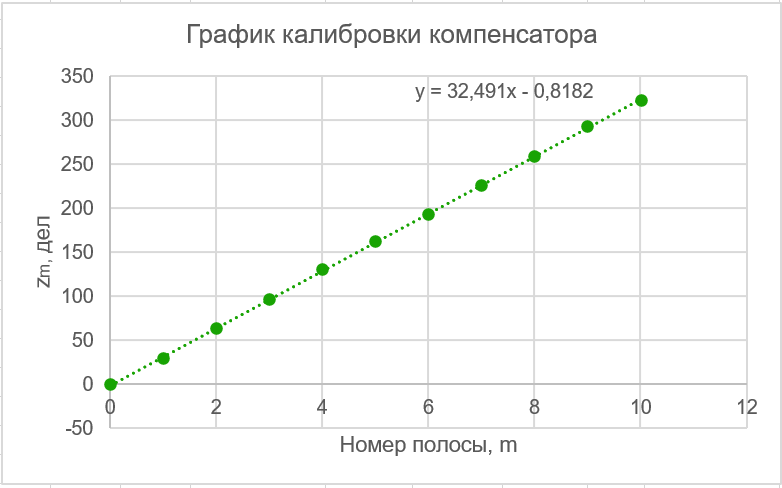
\includegraphics[width=19cm]{calibration.PNG}
    \caption{График калибровки компенсатора}
    \label{img2}
\end{figure}

Длина кюветы $l_{кювета} = 10$ см, а длина волны, пропускаемая светофильтром $\lambda = 620 \div 720$ нм -- в среднем $\lambda \approx 670$ нм. Тогда $32$ деления компенсатора соответствуют $670$ нм. 

\item По формуле перейдём от делений компенсатора к величине $\delta n$:
\begin{equation}
    \delta n = m\frac{\lambda}{l},
\end{equation}
при этом из графика 1: $\Delta m = \frac{\Delta z}{\tg \varphi_1}$, где $\tg \varphi_1 = 32$ -- угол наклона калибровочного графика. Тогда окончательно

\begin{equation}
    \delta n = \frac{\Delta z}{\tg \varphi_1} \frac{\lambda}{l} = 2.1 \cdot 10^{-7} \, \Delta z
\end{equation}

\end{enumerate}

\subsection{Зависимость $\Delta n$ от $\Delta P$ для воздуха}

\begin{enumerate}
    \item Убедились, что давление воздуха в обеих камерах куветы атмосерное. Установили сильфон в среднее положение и отсоединили первую камеру от атмосфера, перекрыв кран $\text{К}_1$.
    \item Изменяя давления с помощью сильфона и совмещая нулевые полосы, сняли зависимость показаний компенсатора $z$ от перепада давлений $\Delta P$. Мы фиксировали давление сразу же, поскольку в последствии давление падало из-за утечек. Результаты представлены в таблице $\ref{tab2}$.

    \begin{table}[h]
        \centering
        \caption{Зависимость показаний микрометра от давления}
        \begin{tabular}{|*{10}{l|}} \hline
            $\Delta P$, мм вод ст & $-800$ & $-700$ & $-600$ & $-500$ & $-400$ & $-300$ & $-200$ & $-100$ &$0$ \\ \hline
            $z$, дел & 179.5 & 194.5 & 209,5 & 222.5 & 235,5 & 252 & 265.5 & 280.5 & 297.5\\ \hline   
        \end{tabular}
        \begin{tabular}{|*{9}{l|}} \hline
            $\Delta P$, мм вод ст & $100$ & $200$ & $300$ & $400$ & $500$ \\ \hline
            $z$, дел & 306.5 & 322.5 & 337.5 & 346.5 & 362.5 \\ \hline   
        \end{tabular}  
        \label{tab2}
    \end{table}

    \begin{figure}[h]
    \centering
    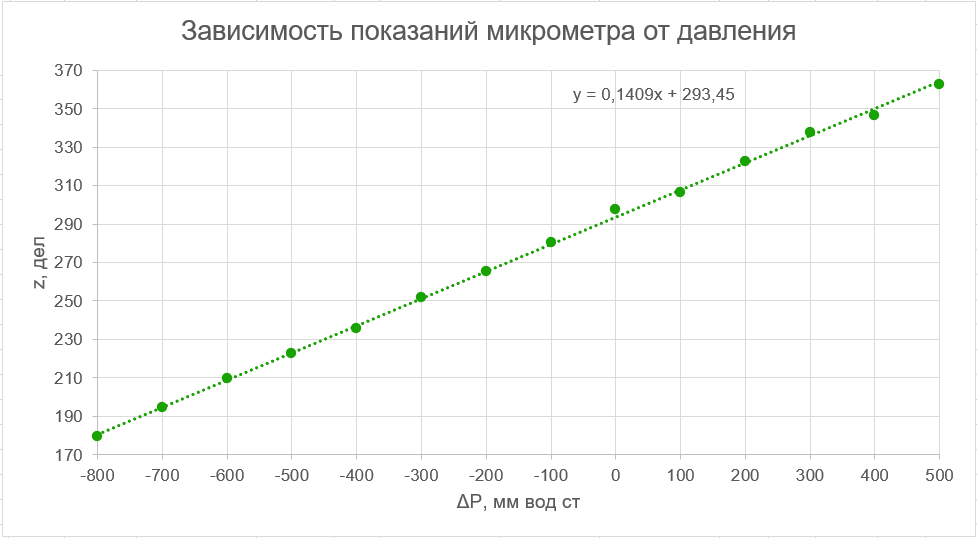
\includegraphics[width=18cm]{deltaP.PNG}
    \caption{Зависимость показаний микрометра от давления}
\end{figure}

Угол наклона графика $\tg \varphi_2 = 0.14 \, \dfrac{\text{дел}}{\text{мм. вод. ст.}}$

\item Определим среднюю поляризуемость молекулы воздуха:

\begin{equation}
\delta n = \frac{2 \pi \alpha}{k_B T} \Delta P
\end{equation}

\begin{equation}
\alpha = \frac{\delta n k_B T}{2 \pi \Delta P} = \frac{\Delta z \lambda}{\tg \varphi_1 l} \frac{k_B T}{2 \pi \Delta P} =\frac{\tg \varphi_2}{\tg \varphi_1} \frac{\lambda k_B T}{2 \pi l} = 192 \cdot 10^{-32}
\end{equation}

\item Определим показатель преломления воздуха по формуле
\begin{equation}
    n_0 = 1 + 2\pi\alpha \frac{P_0}{kT_0} = 1.00032
\end{equation}

Для $T = 292.6$ K и $P = 99.4$ кПа
\begin{equation}
    n = 1 + \frac{(n_0 - 1)T_0 P}{T P_0} = 1.000297
\end{equation}

\item Во вторую кювету запустим углекислый газ. Сразу после этого набежит разность хода, которая компенсируется поднятием компенсатора на 190 мкм.

Так как $n_2 - n_1 = \delta n$, а $\delta n$ была определена по формуле через калибровочный график, $\delta n = \Delta z \frac{\lambda}{l \tg \varphi_1} = 0.995 \Delta z$

Поэтому 
\begin{equation}
    n_{CO2} = n + 0.995\Delta z = 1.000303 + 0.000179 = 1.000482 \pm 0.000032
\end{equation} 
\end{enumerate}

\subsection{Сравнение показателей преломления воздуха и углекислого газа при атмосферном давлении}

\begin{enumerate}
    \item Соединили первую камеру кюветы с атмосферой, открыв кран $\text{К}_1$, и отключили манометр, закрыв кран $\text{К}_2$. Заполнили углекислым газом камеру с открытым концом.
    \item Совместили нулевые полосы. Картина сдвинулась более чем на $25$ полос, что говорит о том, что камера в большей мере заполнена углекислым газом, воздуха в ней почти нет.
    \item Сняли зависимость равновесного положения компенсатора от времени (таблица $\ref{tab3}$), раз в минуту совмещая нулевые полосы, и оценили время установления равновесия $\tau\approx10\text{ мин}$.
    \item Определили температуру $T=19.6\text{ }^{\circ}C$ и давление $P=99.4\text{ кПа}$ по показаниям лабораторного термометра и барометра.

\end{enumerate}

\begin{table}[h]
    \centering
        \begin{tabular}{|c|*{10}{c|}}
        \hline
        $t$, мин & 0 & 1 & 2 & 3 & 4 & 5 & 6 & 7 & 8 & 9 \\ \hline
        $z$ & 10.245 & 9.275 & 8.565 & 8.15 & 7.475 & 6.165 & 5.885 & 5.625 & 5.415 & 5.275 \\ \hline
    \end{tabular}
    \caption{Результаты измерений}
    \label{tab3}
\end{table}

\section{Подведение итогов и выводы}

В ходе данной лабораторной работы мы исследовали изменение показателя преломления воздуха при изменении давления. Для этого мы настроили установку, провели калибровку компенсатора и сняли зависимость показателя преломления от давления. Так же мы определили разность показателей преломления воздуха и углекислого газа при атмосферном давлении. По результатам измерений мы рассчитали показатели преломления соответствующих газов при нормальных условиях:

\begin{center}
    \boxed{ n_{\text{возд}} = (\pm) \text{ }(\varepsilon=\%) }
\end{center}

\begin{center}
    \boxed{ n_{CO_2} = (\pm) \text{ }(\varepsilon=\%) }
\end{center}


\end{document}

